
\chapter{PCB Assembly and Testing}
\vspace{-14mm}
The PCB would be assembled in sections.  All the components required to get a certain aspect of the PCB functioning would be soldered down and then that aspect will be tested. 

\vspace{-1mm}
\textbf{Components to be assembled :}
\begin{figure}[H]
        \begin{enumerate}
        \setlength{\itemsep}{-1.5mm}
        \item Buck converter
        \item Voltage regulator
        \item Temperature sensor
        \item Current sensor
        \item Microcontroller
        \item MAX48
    \end{enumerate}
\end{figure}

\vspace{-8mm}
The voltage regulator, MAX485, temperature and current sensor chips all had simple configurations and when tested worked as expected as seen in chapter 4, Component Testing. The microcontroller and buck converter required a more complicated setup. The two chips and the components necessary for their functioning can be see soldered down in Figure 6.1.

\vspace{2mm}
\begin{figure}[H]
\centering
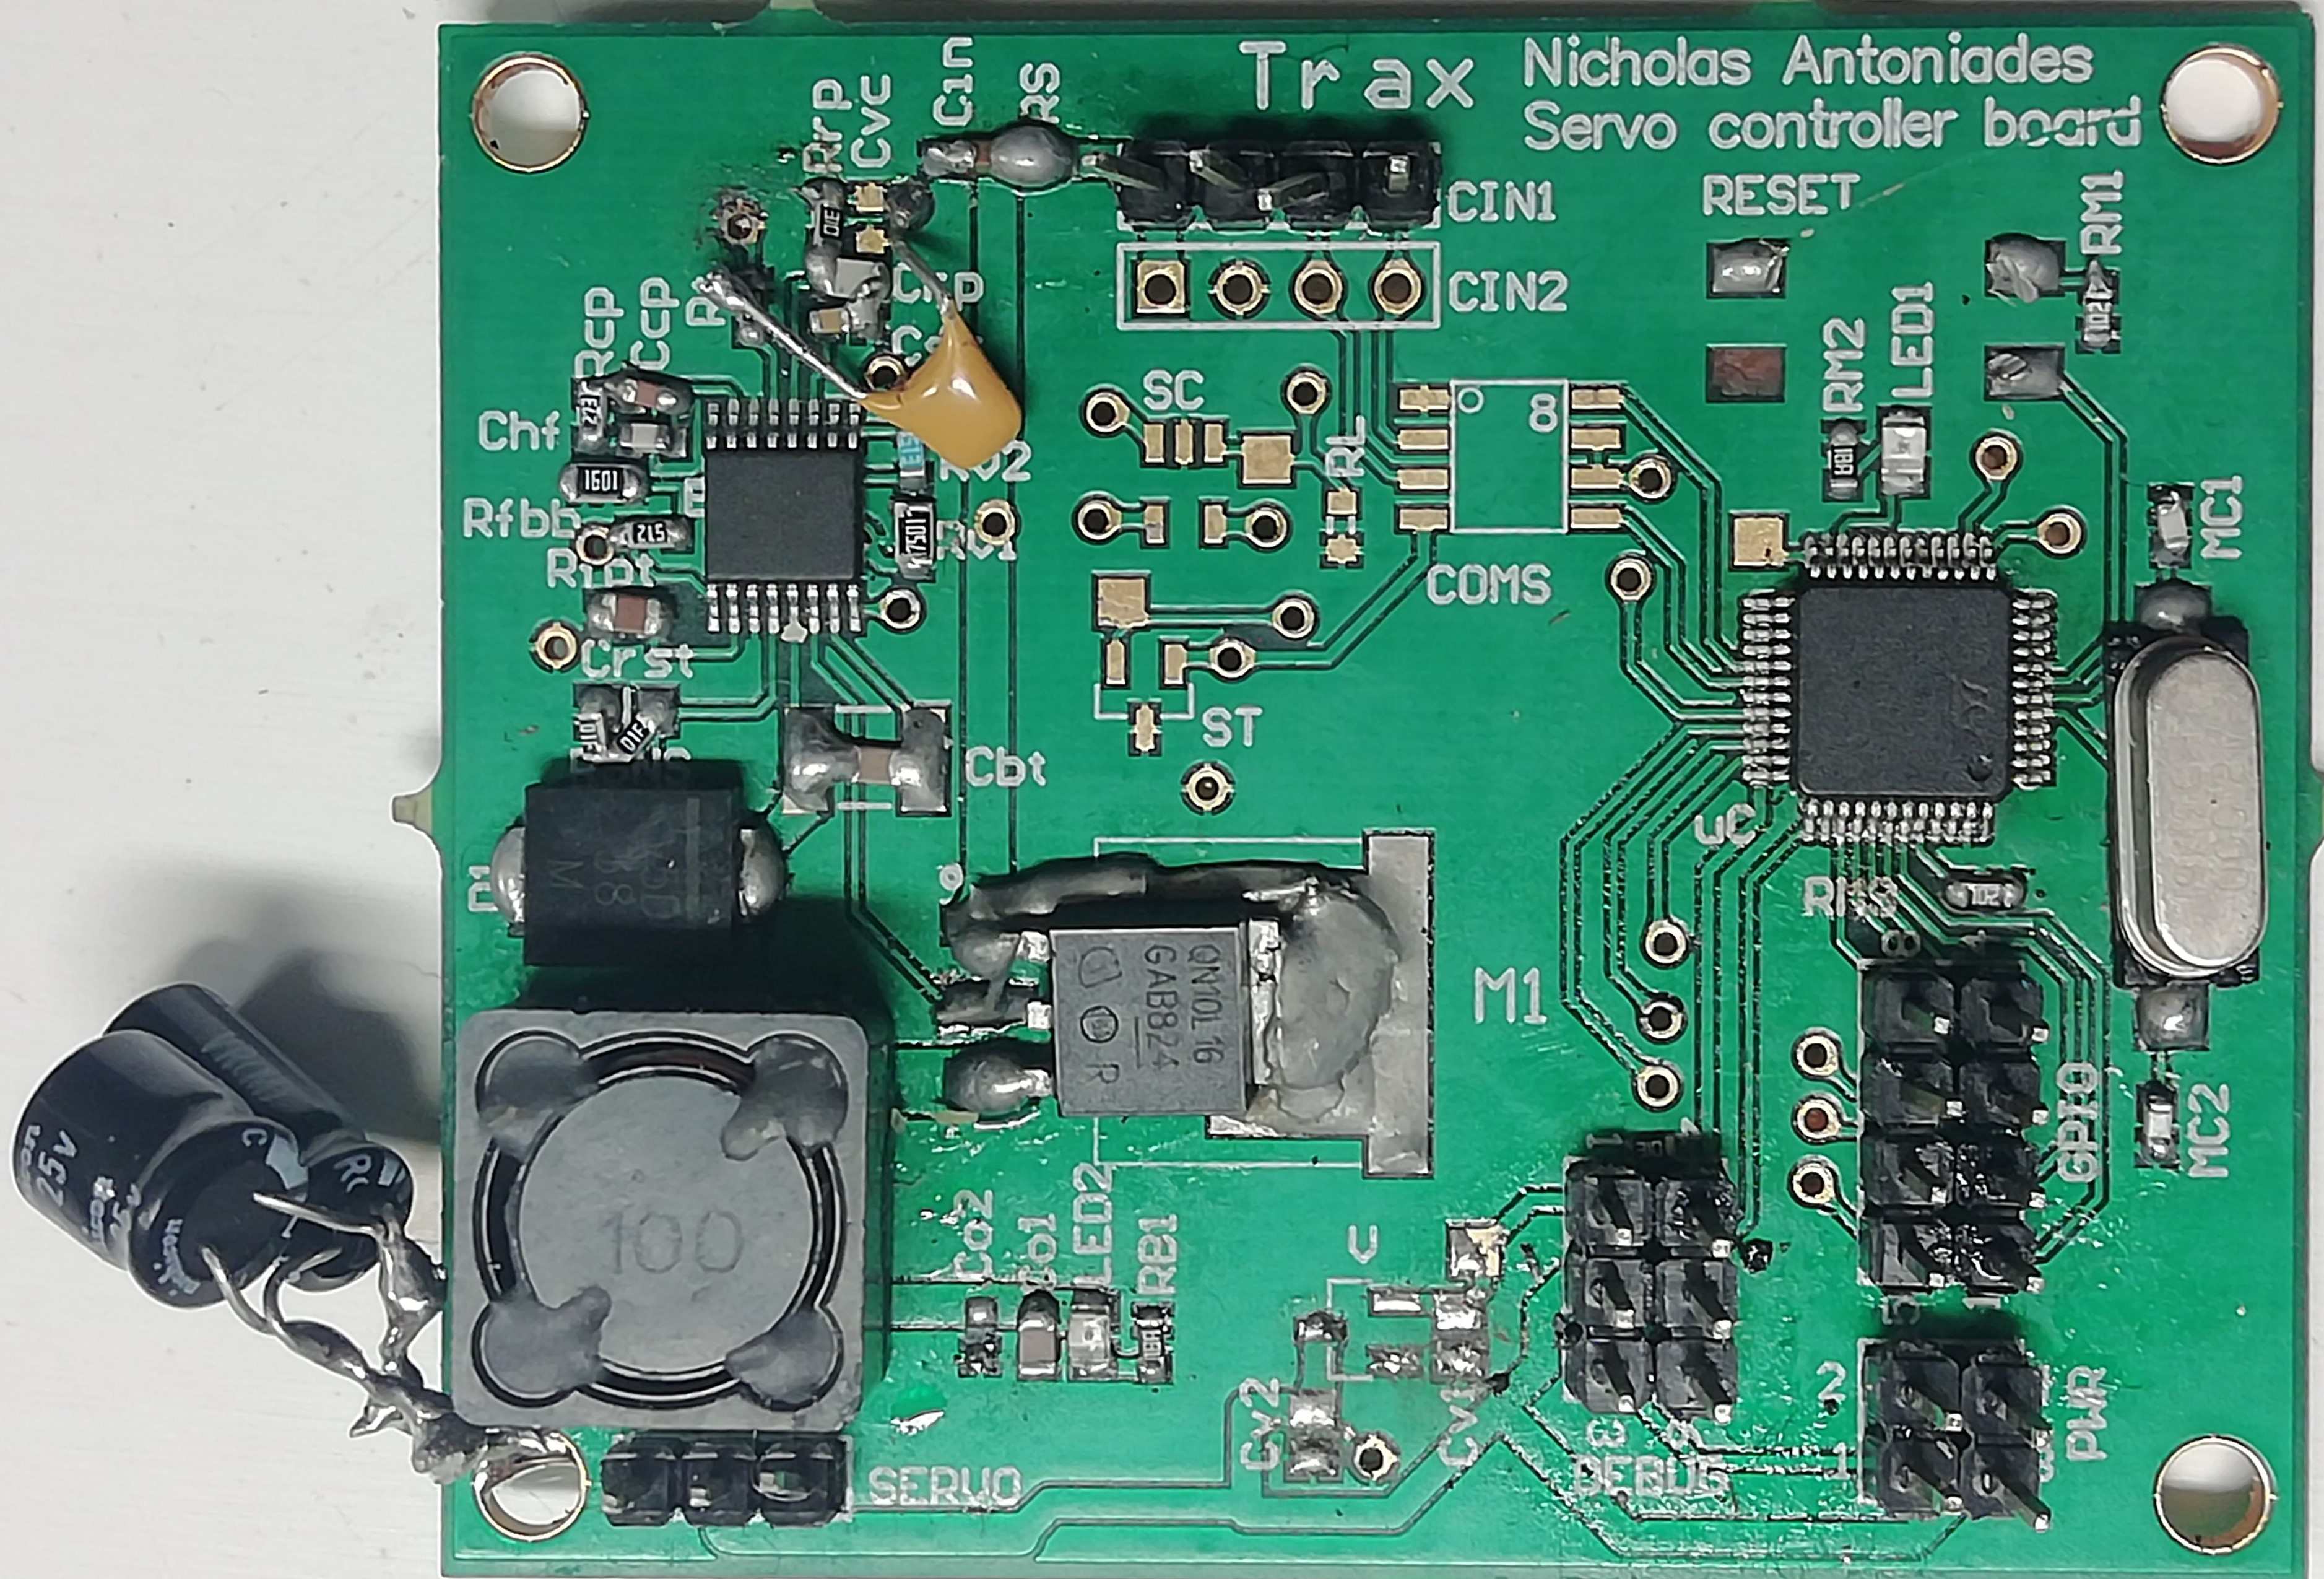
\includegraphics[width=0.8\textwidth]{Soldered_PCB.jpg}
\vspace{-1mm}
\caption{Microcontroller and buck converter on PCB}
\end{figure} 
\vspace{-5mm}

\newpage
\section{Buck Converter}
\vspace{-3mm}
The buck converter chip and all necessary components required for it to function were soldered on to the board. Headers were soldered down enabling the power, ground and output cables to be to connected allowing testing. A couple issues came up when soldering the buck converter to the PCB.
\vspace{-5mm}
\begin{enumerate}
    \item The capacitor values designed for had were only available in the electrolytic packages. The through hole capacitors were soldered to the surface mount pads. 
    \vspace{-3mm}
    \begin{figure}[H]
      \centering
      \begin{minipage}[b]{0.45\textwidth}
        \begin{figure}[H]
            \centering
            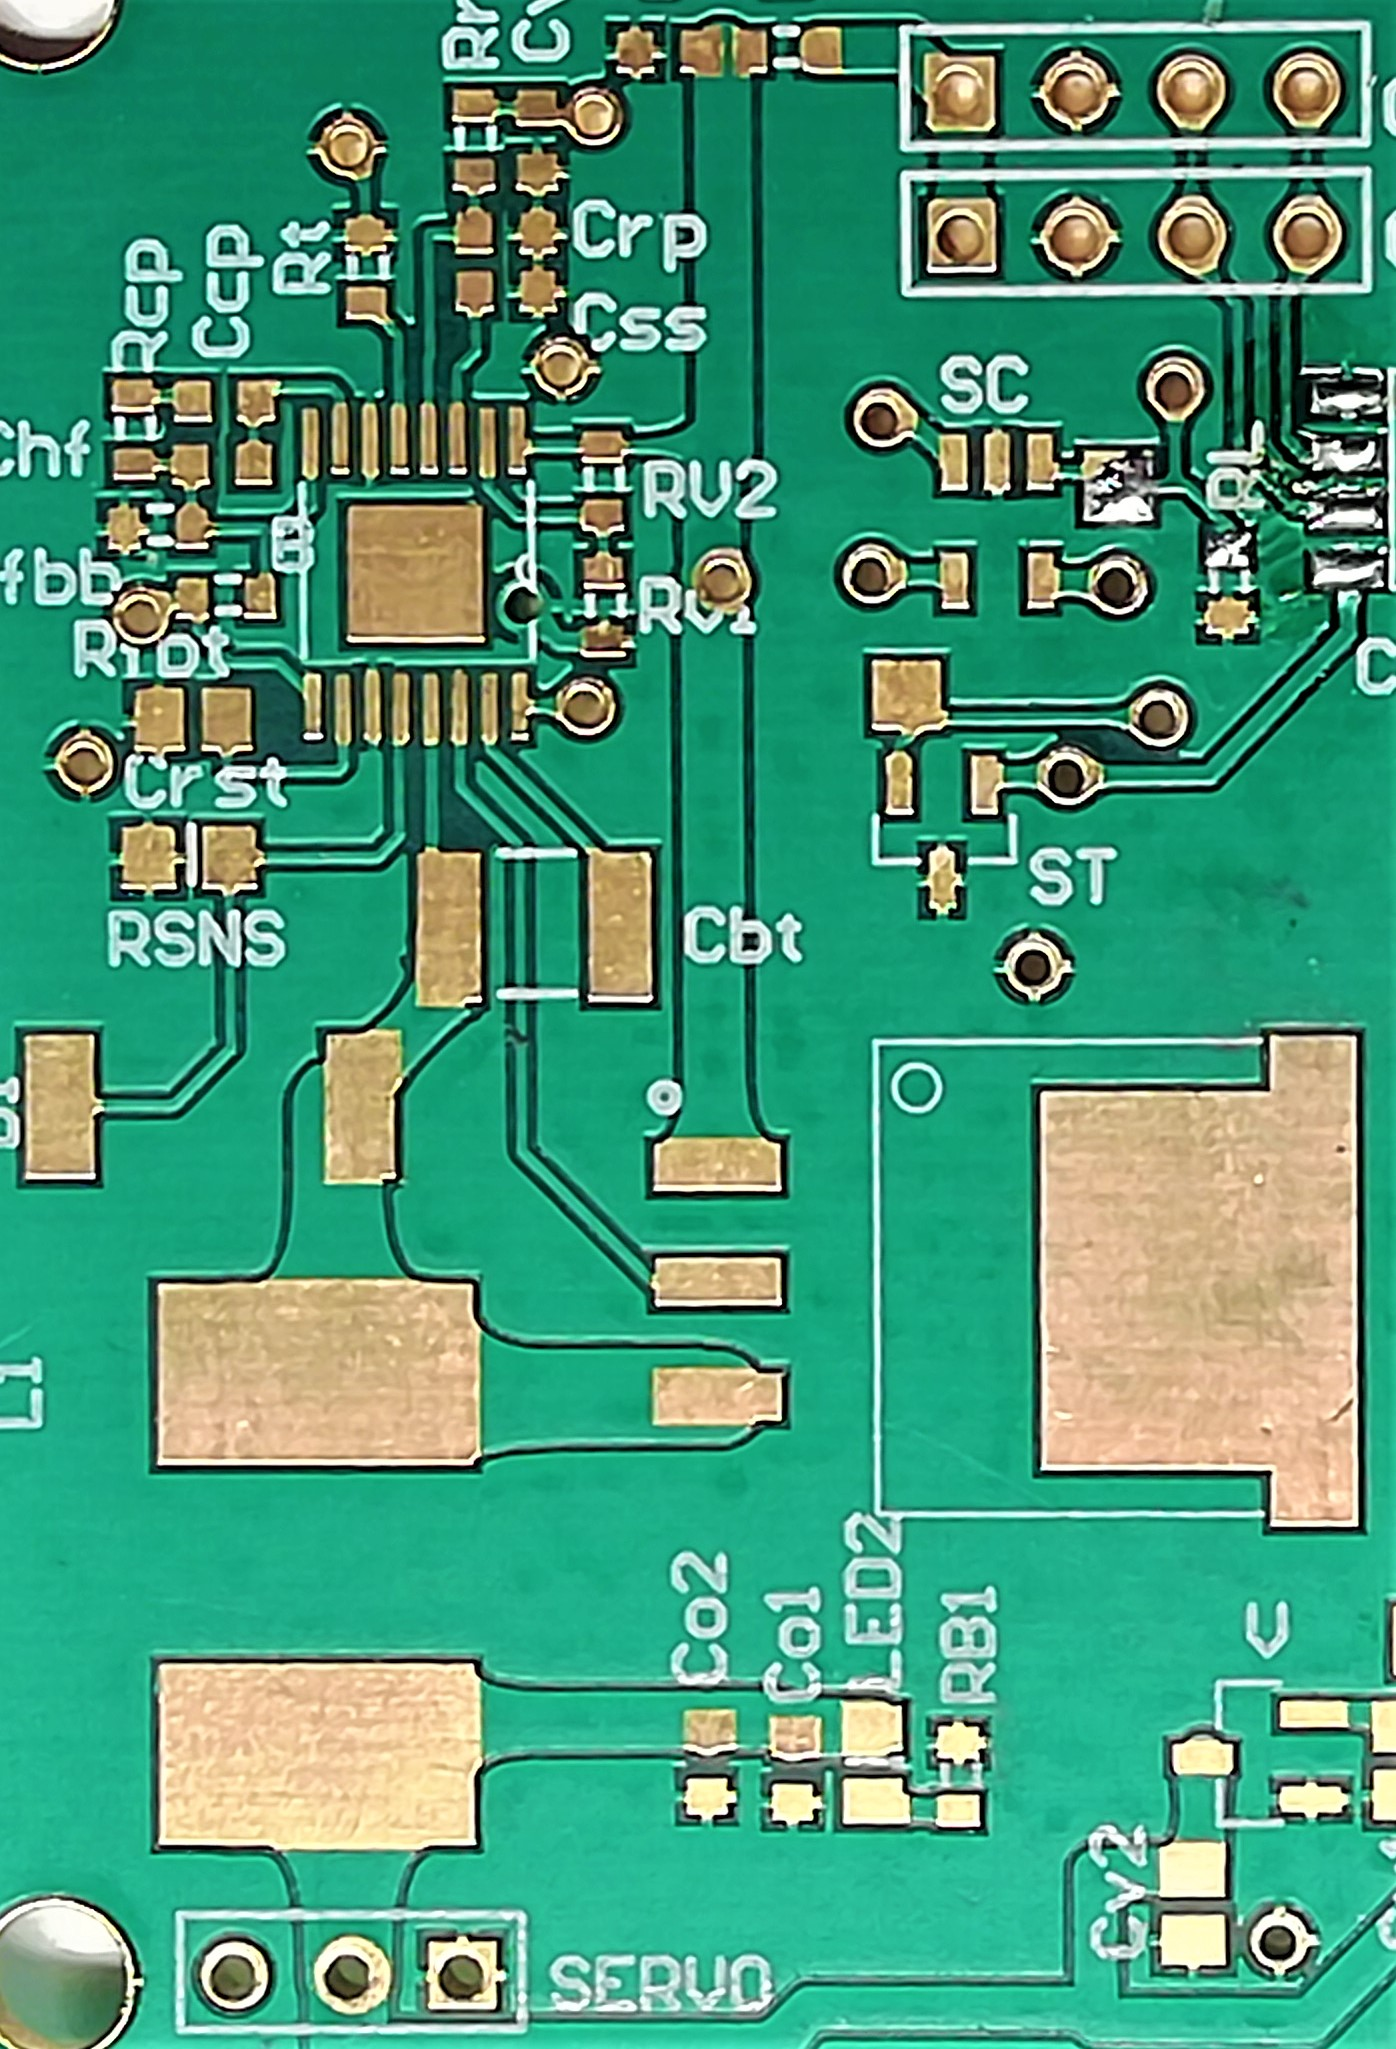
\includegraphics[width=0.62\textwidth]{footprint_buckconverter.jpg}
            \caption{Buck converter footprints}
        \end{figure}
      \end{minipage}
      \hfill
      \begin{minipage}[b]{0.45\textwidth}
        \begin{figure}[H]
            \centering
            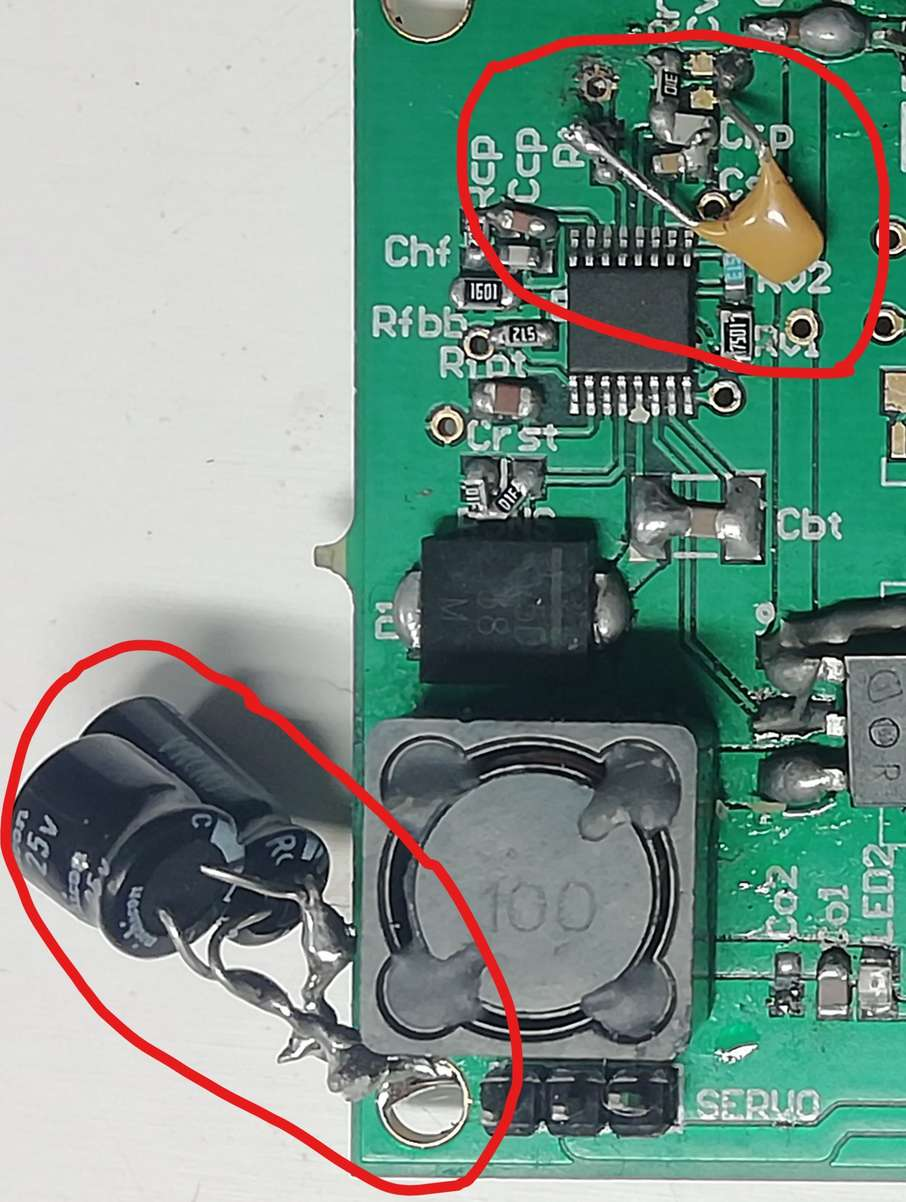
\includegraphics[width=0.7\textwidth]{Solder_capacitors.jpg}
            \caption{LM5088 soldered down}
        \end{figure}
      \end{minipage}
    \end{figure}
    
    \vspace{-5mm}
    \item The MOSFET footprint that was designed had been chosen for a  different MOSFET that was not available from suppliers. The pins of the new MOSFET were in a different order and a wire had to be soldered across the pad so that the in order to allow the MOSFET to be connected correctly. This can be seen in Figures 6.4 and 6.5.
    
    \begin{figure}[H]
      \centering
      \begin{minipage}[b]{0.5\textwidth}
        \begin{figure}[H]
            \centering
            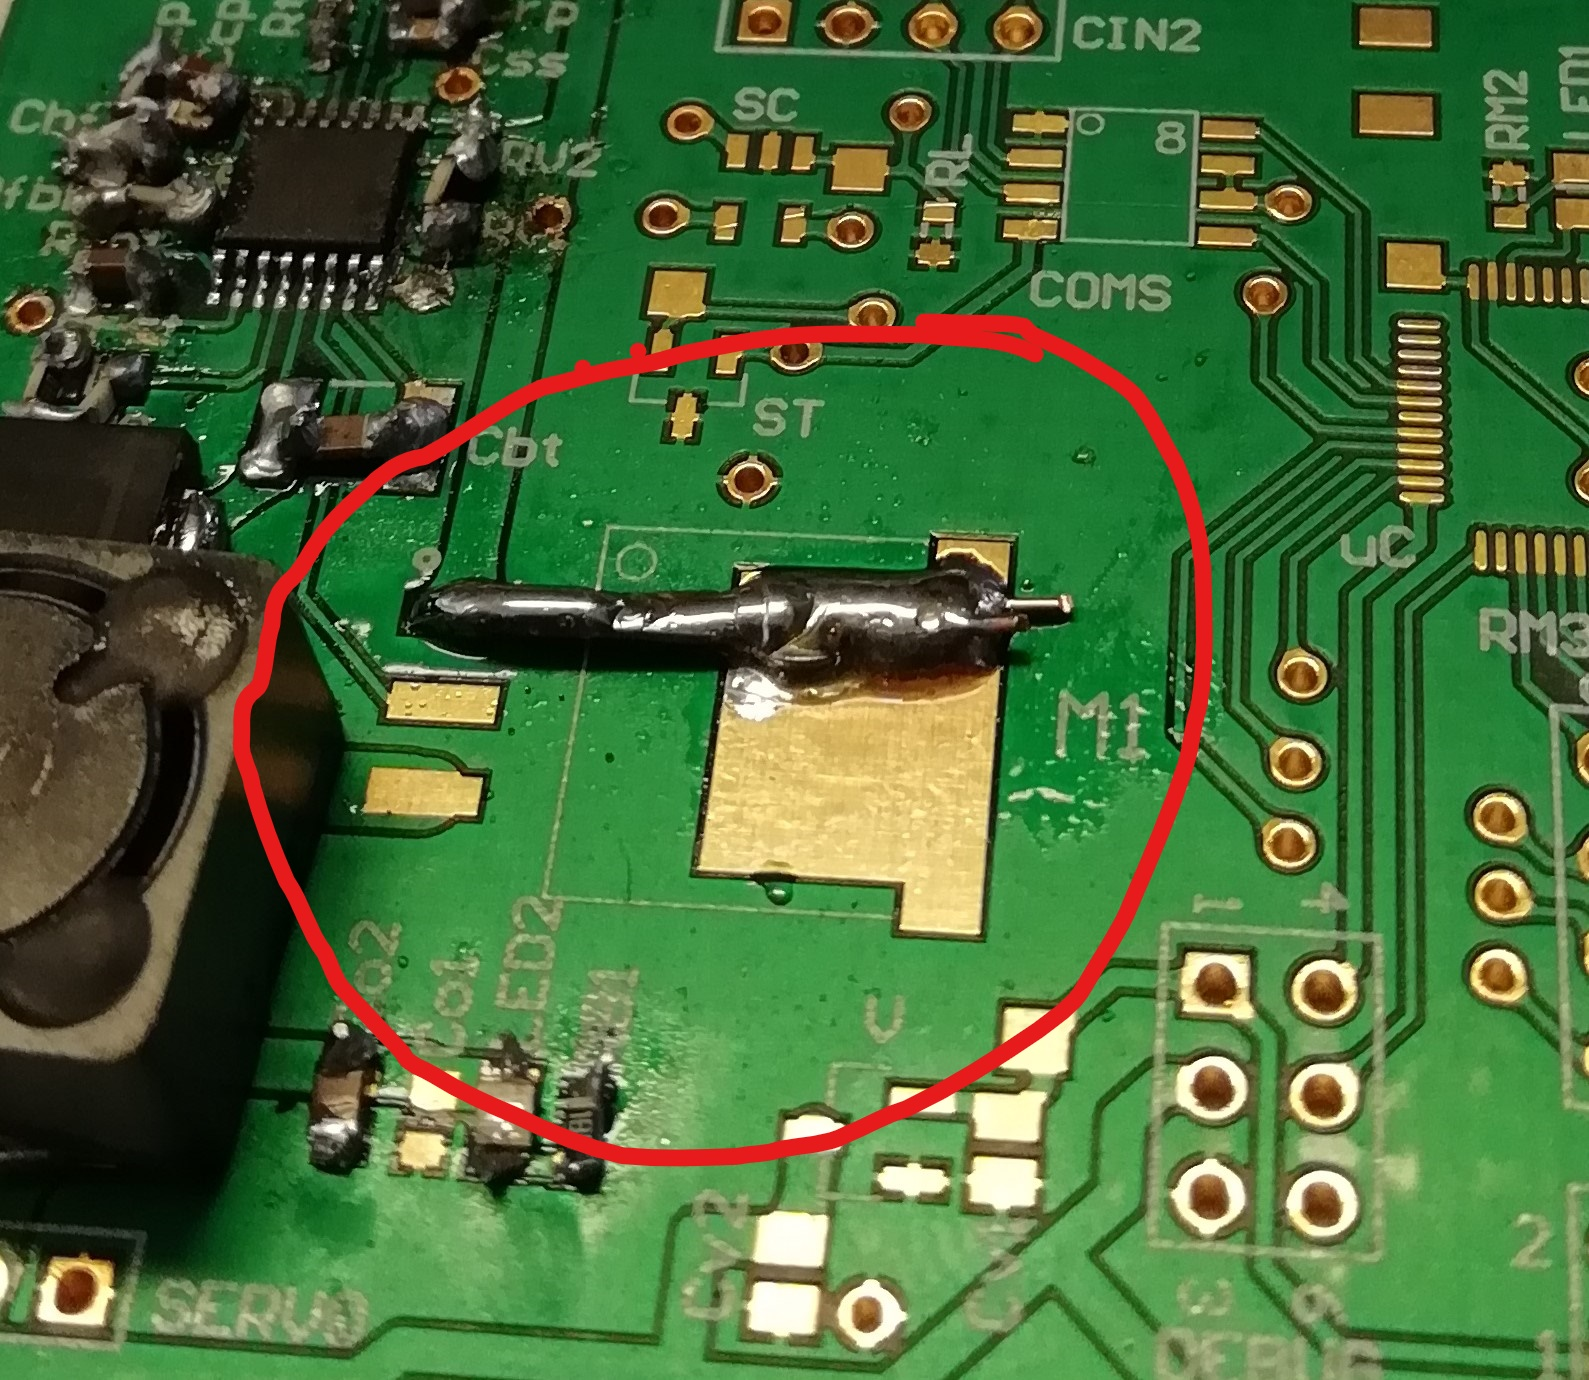
\includegraphics[width=0.7\textwidth]{Solder_mosfet.jpg}
            \caption{Correcting MOSFET}
        \end{figure}
      \end{minipage}
      \hfill
      \begin{minipage}[b]{0.45\textwidth}
        \begin{figure}[H]
            \centering
            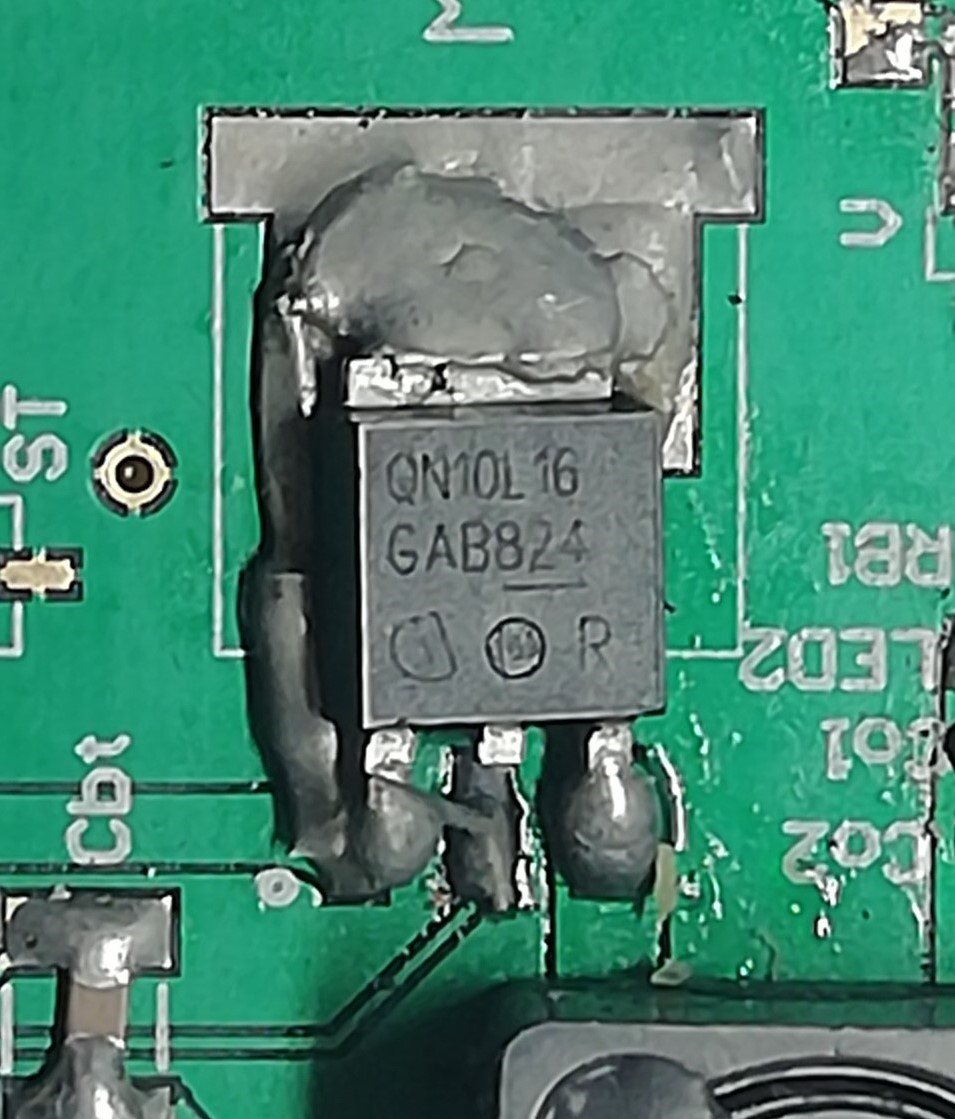
\includegraphics[width=0.6\textwidth]{Solder_mosfet2.jpg}
            \vspace{-3mm}
            \caption{MOSFET soldered down}
        \end{figure}
      \end{minipage}
    \end{figure}
    \vspace{-3mm}
    \item When designing the footprint, no solder mask was inserted between the pins of the buck chip. The result of this was when soldering, solder leaked over creating shorts, as well as letting pins getting close enough to arc. Seen in Figures 6.6 and 6.7.
    
    \begin{figure}[H]
      \centering
      \begin{minipage}[b]{0.5\textwidth}
        \begin{figure}[H]
            \centering
            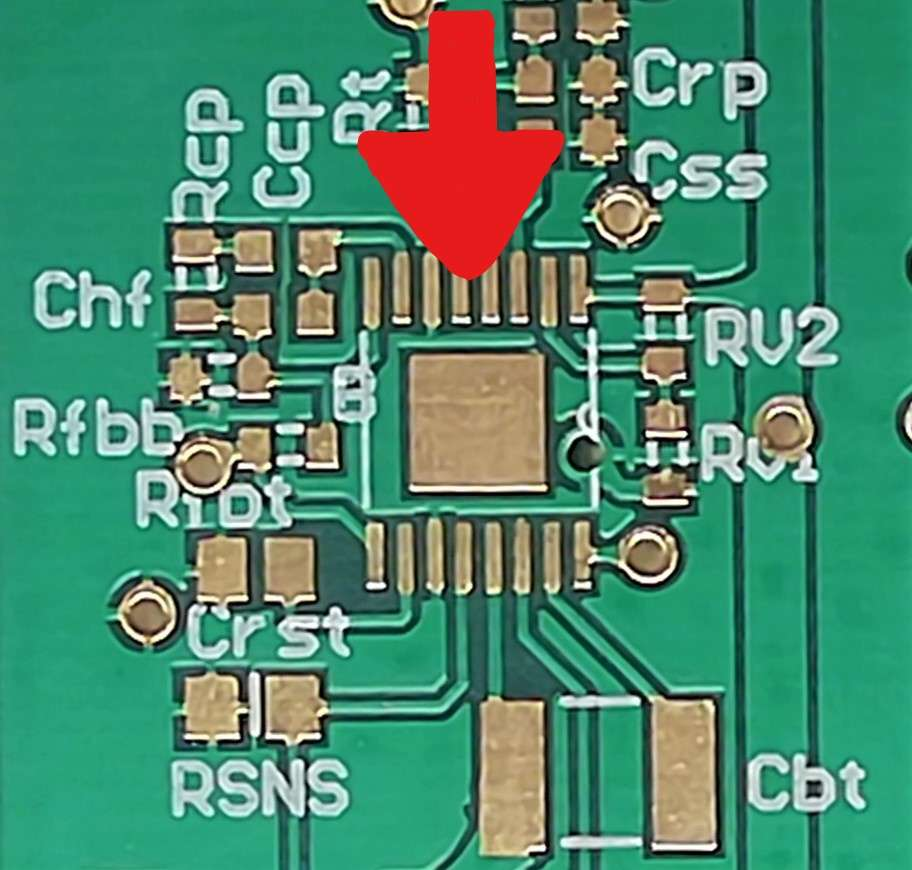
\includegraphics[width=0.7\textwidth]{footprint_buck.jpg}
            \caption{LM5088 footprint}
        \end{figure}
      \end{minipage}
      \hfill
      \begin{minipage}[b]{0.45\textwidth}
        \begin{figure}[H]
            \centering
            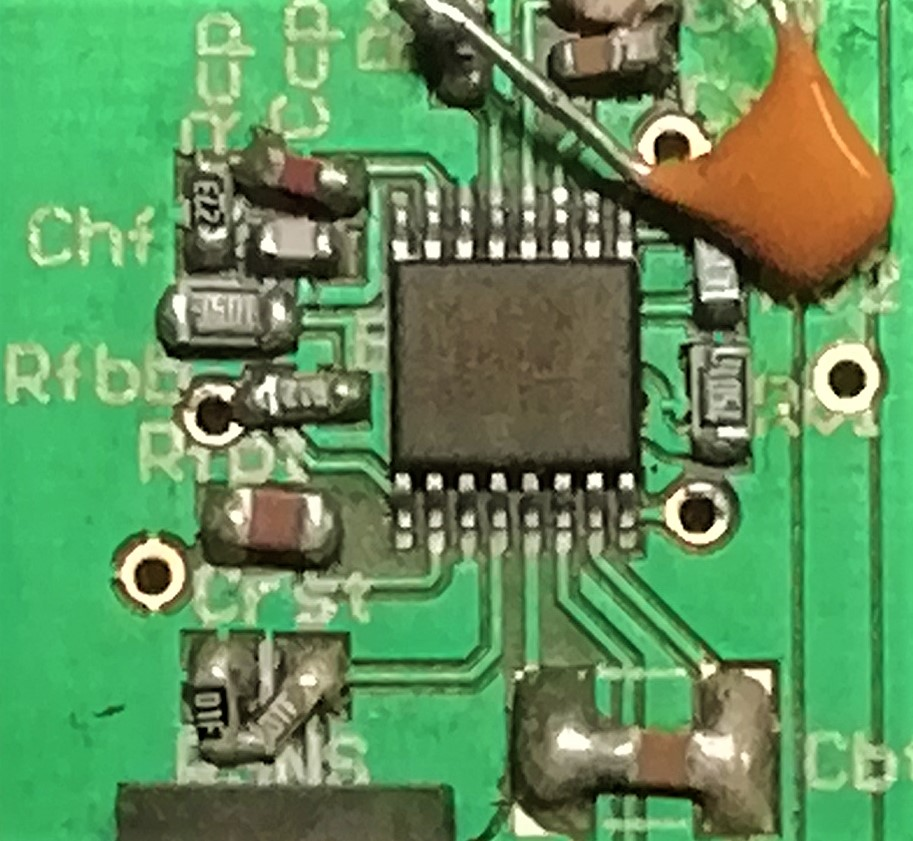
\includegraphics[width=0.83\textwidth]{Solder_buck.jpg}
            \vspace{-3mm}
            \caption{LM5088 soldered down}
        \end{figure}
      \end{minipage}
    \end{figure}
\end{enumerate}


\section{Microcontroller}
\vspace{-5mm}
The STM chip, clock, an indicator LED and necessary resistors and capacitors were placed on the board. Headers were soldered down enabling the power, ground and debugging cables to be to connected. 

The same mistake that had been made in the buck converter footprint design was made for the microcontroller. When connected to power and ground, the pins would short stopping the circuit from working. This can be seen in Figures 6.8 and 6.9.

\vspace{-2mm}
\begin{figure}[H]
  \centering
  \begin{minipage}[b]{0.45\textwidth}
    \begin{figure}[H]
        \centering
        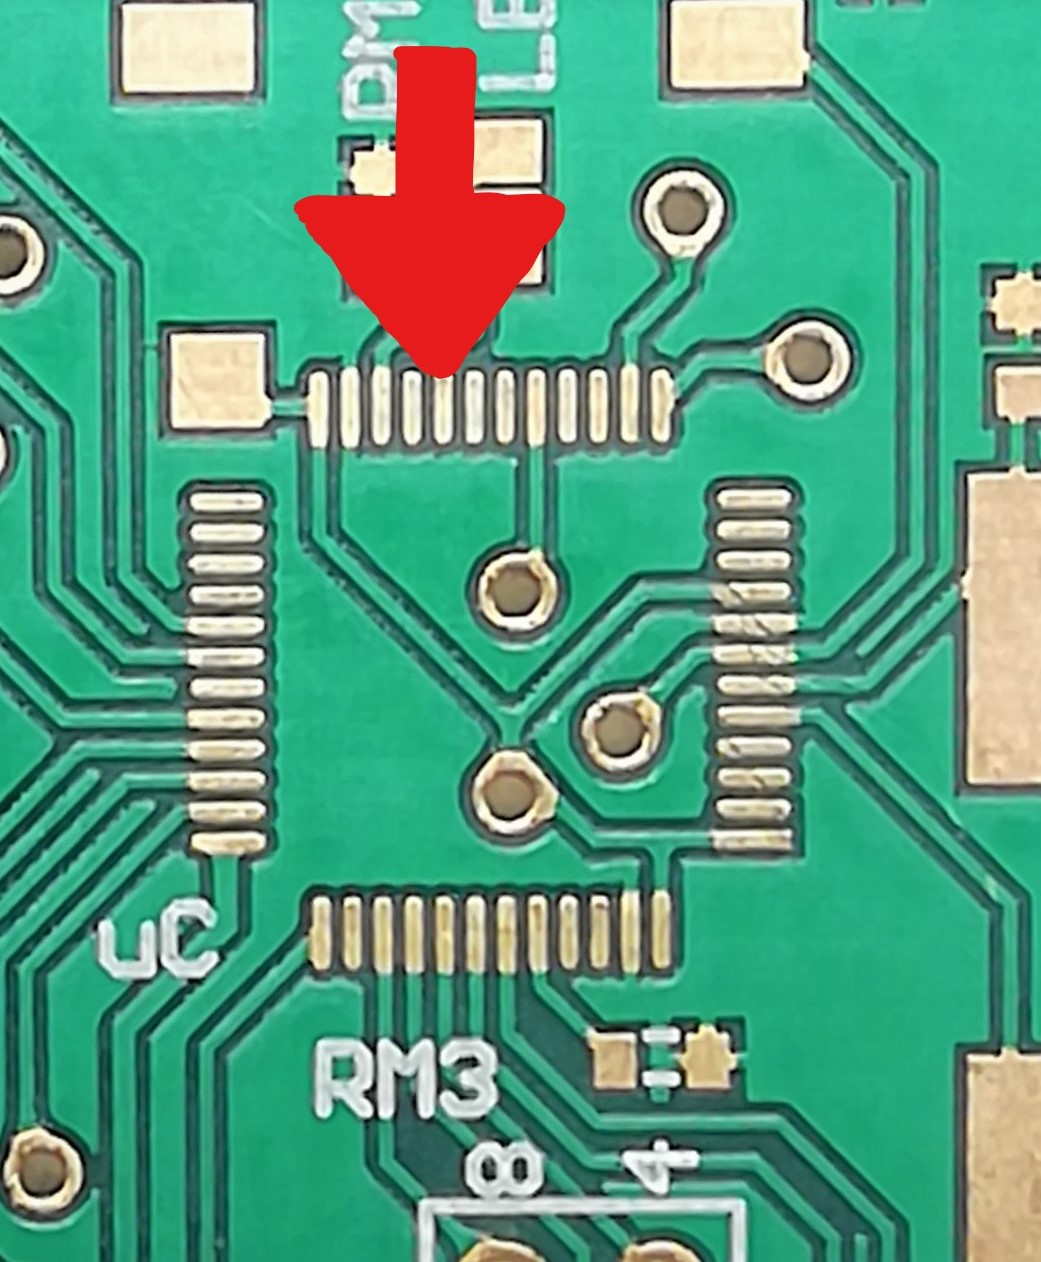
\includegraphics[width=0.7\textwidth]{footprint_micro.jpg}
        \caption{STM footprint}
    \end{figure}
  \end{minipage}
  \hfill
  \begin{minipage}[b]{0.45\textwidth}
    \begin{figure}[H]
        \centering
        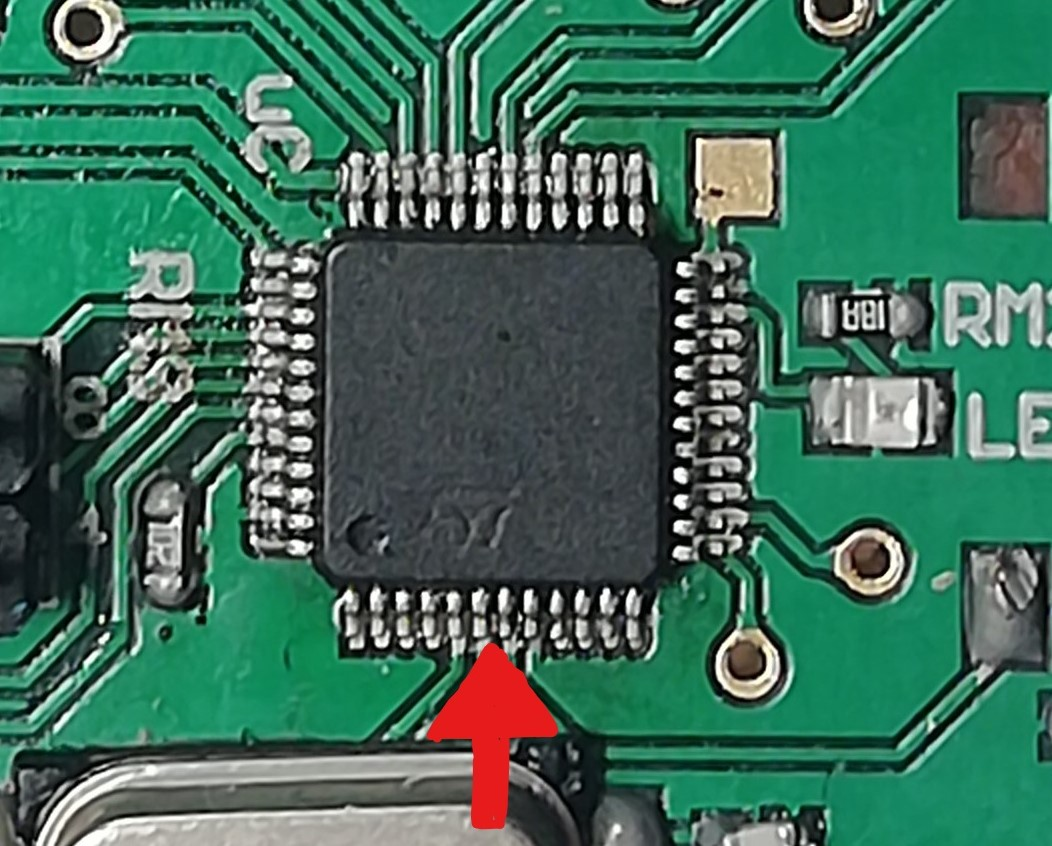
\includegraphics[width=1\textwidth]{Solder_micro.jpg}
        \vspace{-2mm}
        \caption{STM soldered down}
    \end{figure}
  \end{minipage}
\end{figure}





